\documentclass{article}

\usepackage{setspace, tipa, hyperref, graphicx, blindtext, csquotes, textcomp, wrapfig, placeins, tikz, geometry, booktabs, array}
\usepackage[utf8]{inputenc}
\usepackage[english]{babel}
\pagestyle{empty}
\rmfamily
\usepackage[normalem]{ulem}
\usepackage[headsepline]{scrlayer-scrpage}
\clearpairofpagestyles
\ohead{Papineau}
\cfoot{\pagemark}
\ihead{\textbf{Gender Ideology, Production, and Processing}}
\hyphenpenalty=0
\usepackage[backend=biber,style=apa]{biblatex}
\DeclareNameAlias{sortname}{family-given}
\addbibresource{qp1.bib}
\usepackage{gb4e}
%\sloppy
\title{\vspace{-3cm}The Role of Individuals' Gender Ideology on the Production and Processing of Gendered Occupational Titles\\}

\author{B. Papineau}
\date{}
\pagenumbering{roman}
\setlength\parindent{15pt}

\begin{document}
	
	\maketitle
	\begin{center}
		\textbf{Supervisor: Dr. Rob Podesva}\\
		\textbf{Committee Members: Dr. Judith Degen \& Dr. Meghan Sumner}\\
		\textbf{Word Count: 0000}\\
		\textbf{Date of Submission: Autumn 2021}\\
		\vspace{1cm}
		\textit{In partial fulfillment of the requirements for Doctor of Philosophy in Linguistics at Stanford University}
	\end{center}
	
	\vspace{1.5cm}
	\begin{center}
		\centering
		
\includegraphics[scale=1]{SUSig_Black_Seal_Center.png}
	\end{center}
	
	\newpage
	
	\tableofcontents
	
	\newpage
	\pagenumbering{arabic}
	\setcounter{page}{1}
	
	\section{Introduction}
	
	\subsection{Hypotheses \& Predictions}
	
	\newpage
	\section{Background}
	
	\subsection{Sexism}
	Here I will define the sexism, and also explicate modern ways of measuring it, including \textcite{baber2006social}'s Social Roles Questionnaire.
	
	\subsection{Gender in the English Language}
	
	I will also describe the historical disappearance of gender in the English Language, whose vestiges can be seen almost exclusively in animate-referring pronominals and particular compounds, which form the basis of the present investigation. However, it is also worth noting that the gendered pronouns continue to be employed in non-standard uses for inanimate objects, as described in Suzanne Wagner's PhD dissertation \parencite{wagner2003gender}.
	
	\subsection{Surprisal Theory and Extrasentential Context}
	
	Here is where I will cite \parencite{levy2008expectation}, highlighting and explicating both surprisal theory as a general account for processing and also explicitly invoking the role of extrasentential context, as defined in the work.
	
	\subsection{Gender as an Object of Psycholinguistic Analysis}
	
	Here we will discuss both \textcite{pozniak2021failures} and \textcite{von2020implicit}, which discuss the role of individual beliefs in the marking and processing of gender in the elections of the United States, United Kingdom, and France, in the last five years. They found only a production difference, but none in the perception tasks. Also, I think this was only true for the British contexts.
	
	On the non-morphological, discourse-level, \textcite{hilton2022} found that speakers perceived women to be less friendly than their male counterparts when interrupting interlocutors. This held even with carefully-controlled-for overlap timings, pragmatic and semantic contexts, etc.
	
	We can also discuss \textcite{sarrasin2012sexism}, which found across three different languages that those individuals who held more traditionally sexist beliefs were anti-gender-neutral language reforms more strongly than were those who held more progressive ideologies about gender and equality. This held across three different kinds of sexism (benevolent, hostile, neutral?)
	
	\textcite{gygax2008can} found that blah blah blah French doesn't have true neutrals when using the masculine gender. Similarly, we can cite \textcite{misersky2014norms} and their work on `role nouns', which were normed for gender beliefs (but in a more real-world paradigm). These were both occupational titles (bookkeeper) and what they termed `social roles' (teenager, murderer).

	\newpage
	\section{Norming Study}
	
	\subsection{Methods}
	
	\subsubsection{Participants}
	100 participants were recruited through the online participant recruitment platform \textcite{prolific}. All participants were self-identified L1 English speakers and were born and resided in the United States. None of the participants had participated in the pilot of the norming study. \par
	All participants, regardless of their data's final inclusion in the analysis, were compensated \$2.00 for their participation in the study. The average completion time was 4.353 minutes, which resulted in an average payout of \$31.86/hr.
		
	\subsubsection{Materials}
	For the norming study, we selected 39 `role nouns' \parencite{misersky2014norms} which display overt gender realizations in English. These items were selected from lists of such words, most of which were written specifically to highlight the gendered nature of many occupational titles in English (see for example Kelly 2018). The majority of these forms (29/39) have three differently-marked forms, reflecting the male and female binary genders, as well as a purportedly gender-neutral alternative. Others have only two forms, due to the historically male form being semantically extended to include female referents as well. Examples of both these varieties, as well as some sub-varieties, are included in the Table Below.
	
	\subsubsection{Procedure}
	After providing their informed consent, participants were presented with 20 randomly-ordered sentences of the format ``Someone is a [TITLE]." They were then asked to indicate on a 7-point Likert Scale how likely they thought that the `someone' in question was a man or a woman. Which ends of the scale indicated maleness or femaleness were randomized between participants. Finally, an optional checkbox allowed participants to indicate if they were unfamiliar with a given term. An example of a stimulus slide is provided in Figure X. 
	
	\begin{figure}[h!]
		\centering
		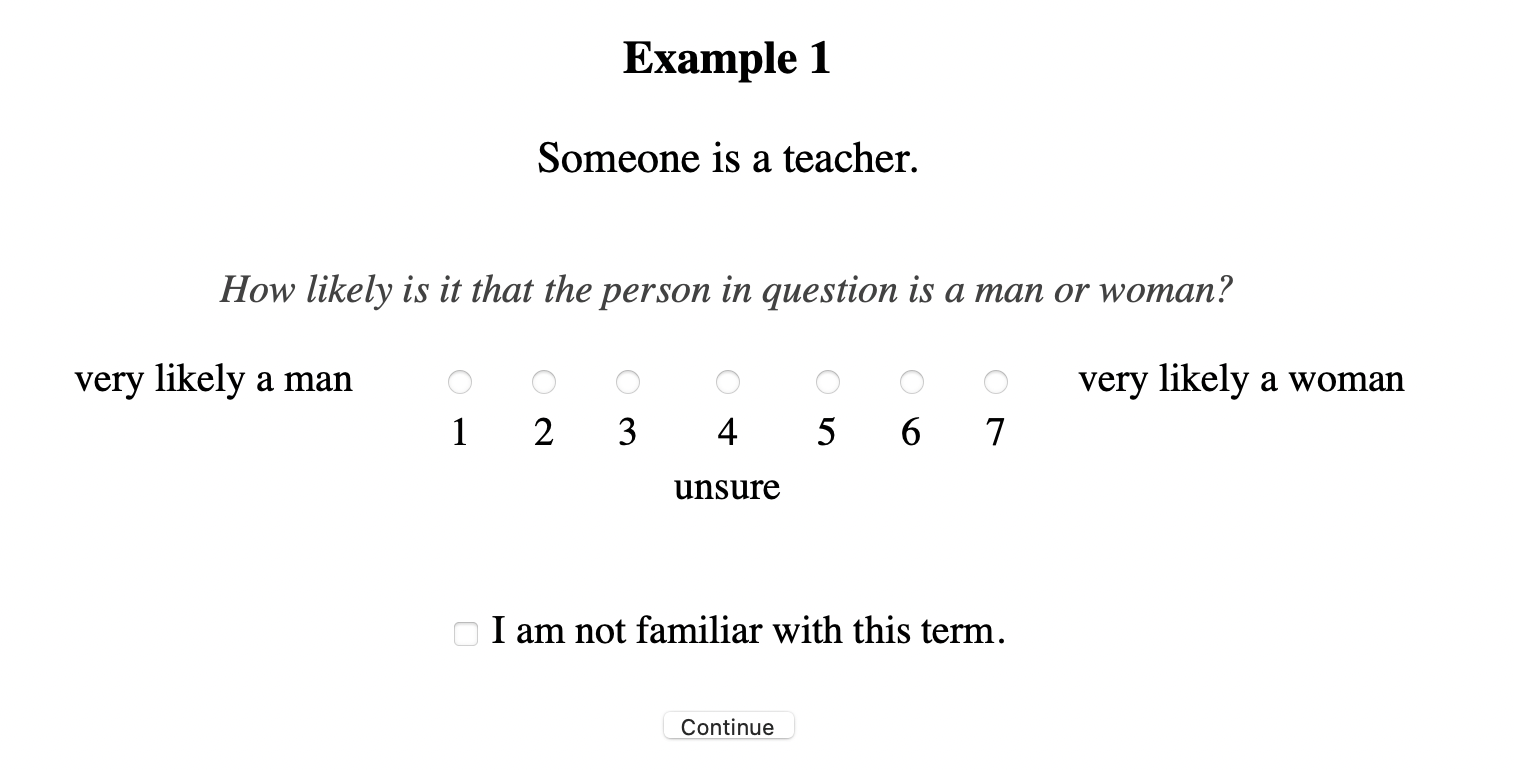
\includegraphics[scale=0.5]{norming_capture}
		\caption{A screenshot of the norming study procedure, as seen by participants}
	\end{figure}

	Participants were given an example trial (as seen above), and then proceeded to the main testing phase of the study. In this phase, each participant saw each of the critical terms once, in one of its three permutations (male, female, neutral). This resulted in 40 trials per participant.\par 
	After the main trial portion of the study, participants filled out an optional demographic and post-experiment survey.
	
	\subsubsection{Exclusions}
	We excluded participants whose average rating for the female terms deviated more than two standard deviations from the sample mean. This was done because, since all the feminine nouns in the materials are morphologically marked as such, we expect near-ceiling responses on the relative female-ness of these terms. We found this to be largely the case (see Figure 2 below), and this criterion resulted in 11 participants being excluded from the analysis.\par 
	We additionally excluded one participant who indicated in the post-experiment survey that they did not understand the task. This resulted in a total of 88 participants being included in the final data analysis.  
	
	\subsection{Results}
	
	\begin{figure}[h!]
		\centering
		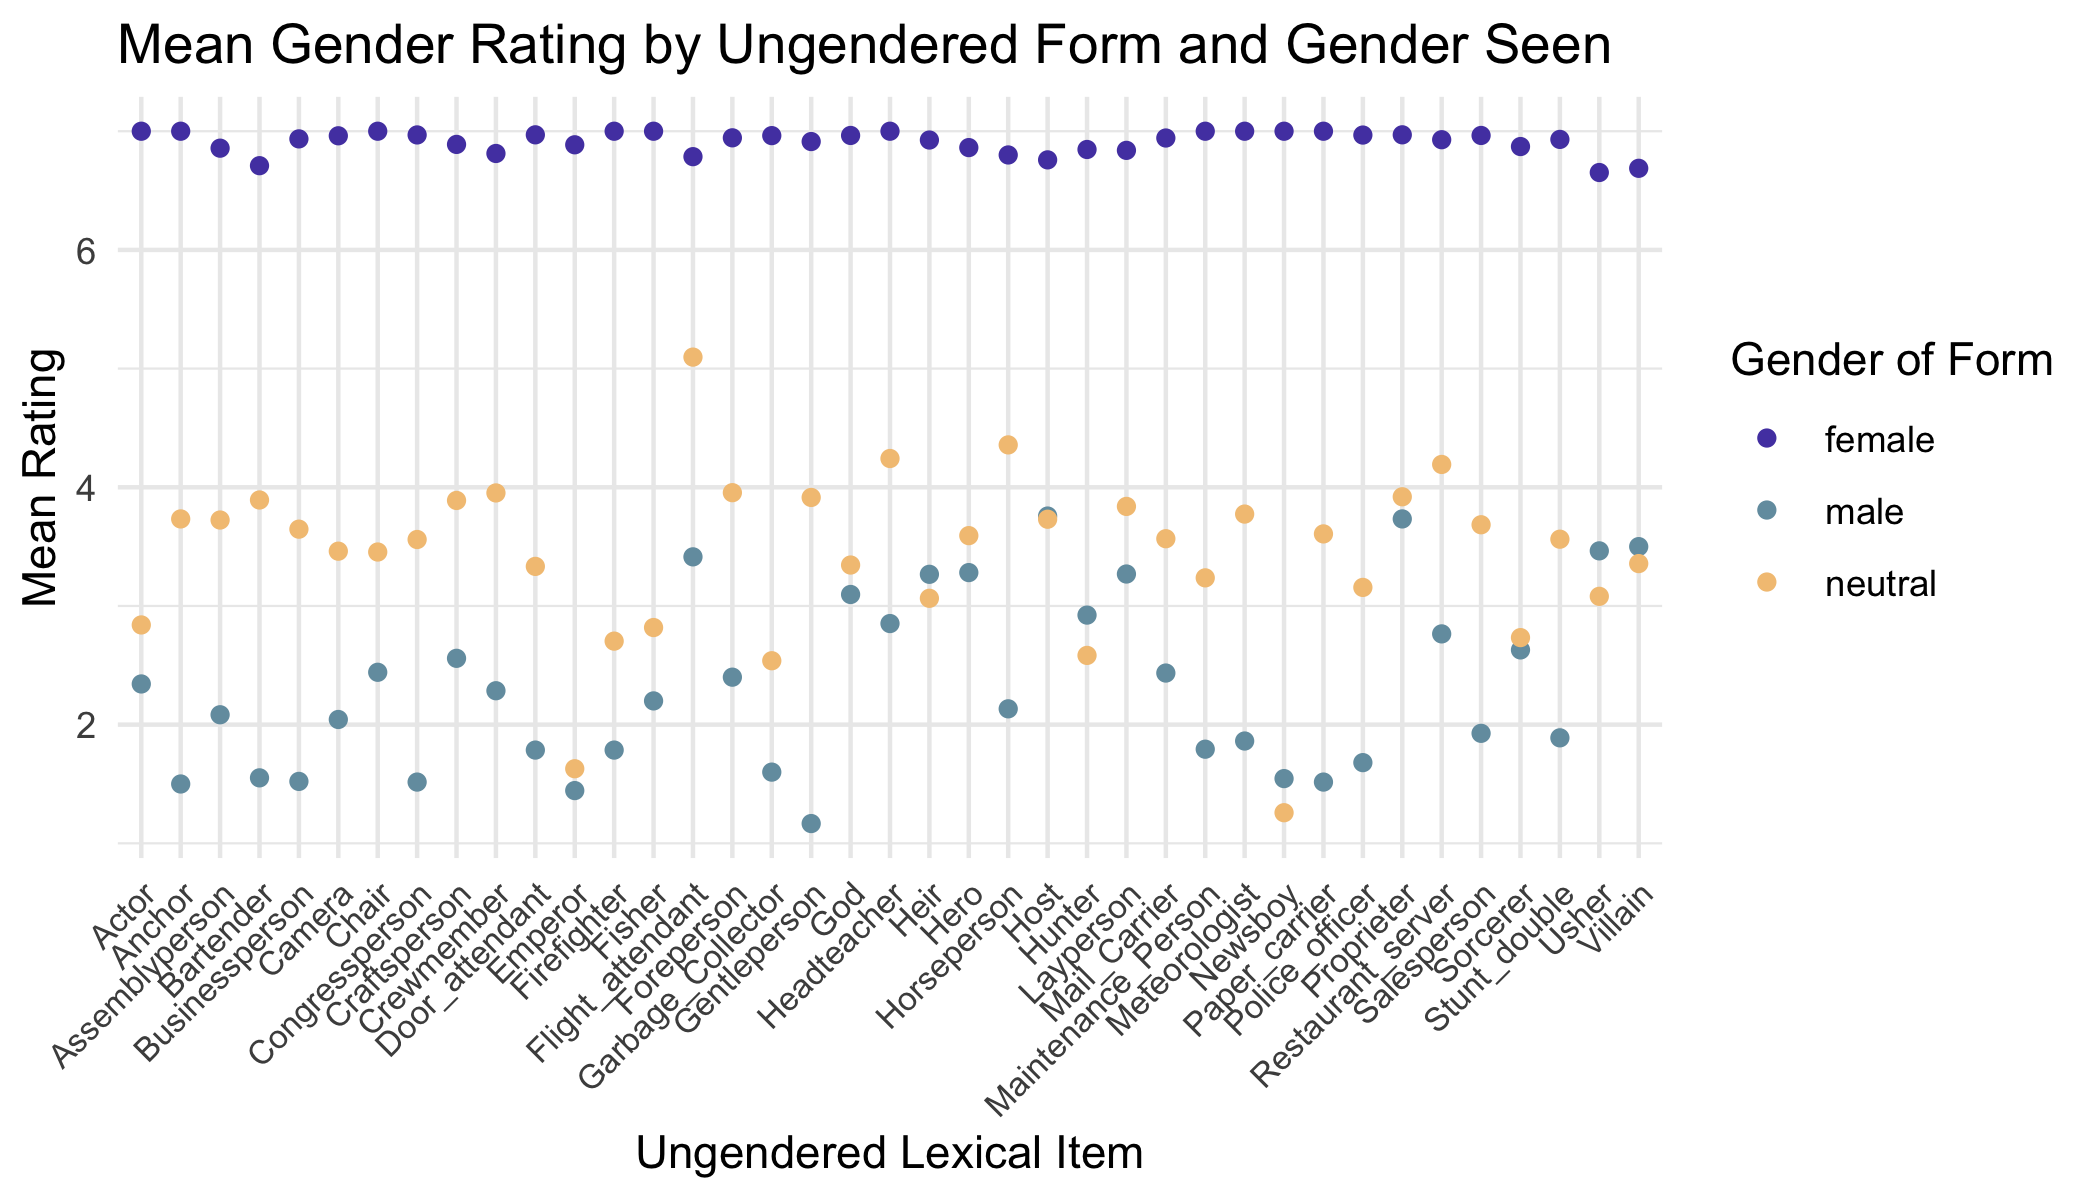
\includegraphics[scale=0.2]{norming_values.png}
		\caption{Mean gender ratings for the items in the norming study. A score of 7 indicates "very likely a woman", while a score of 1 indicates "very likely a man".}
	\end{figure}
	
	\begin{figure}[h!]
		\centering
		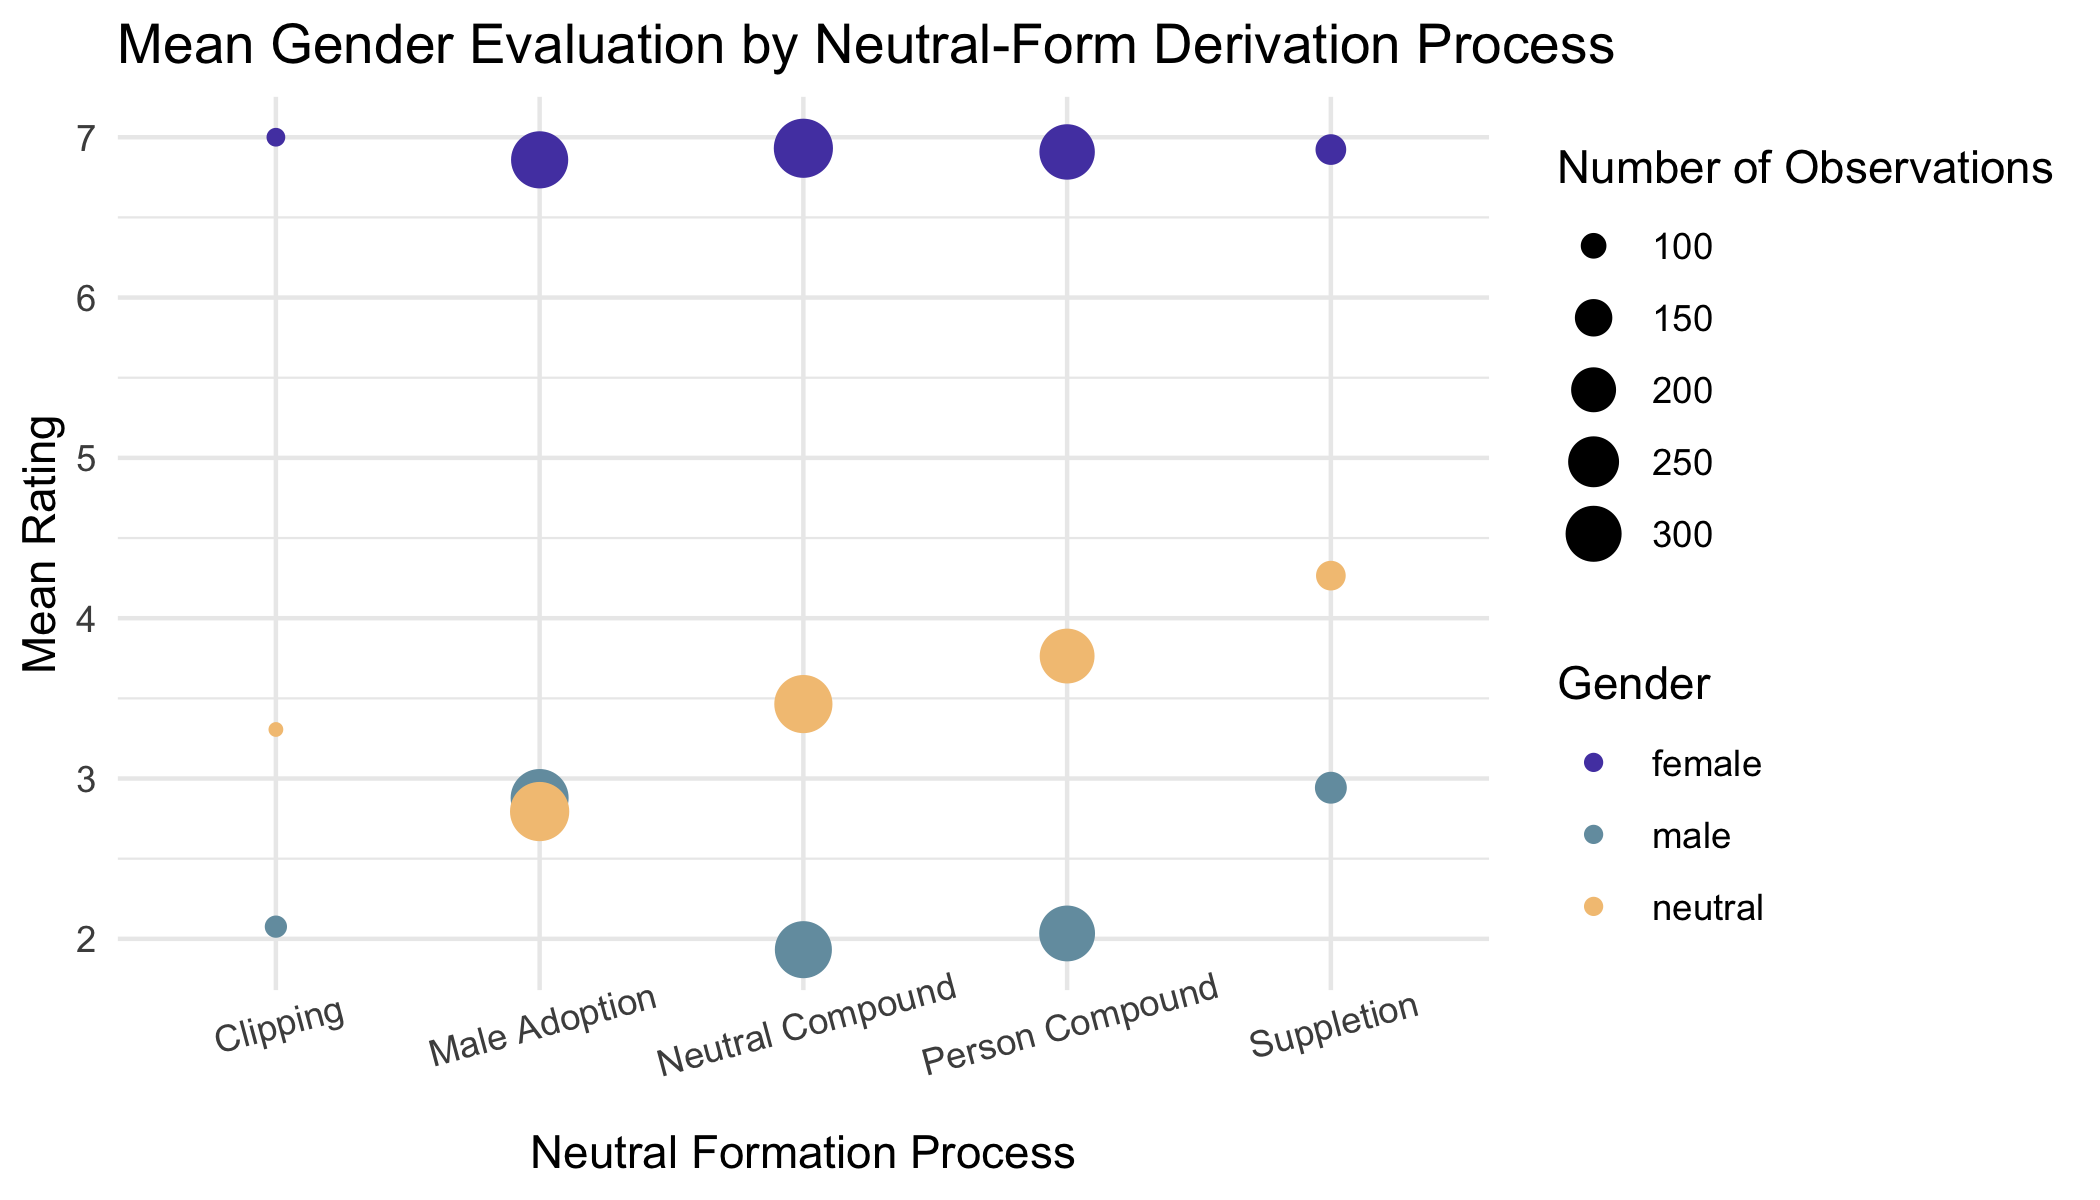
\includegraphics[scale=0.2]{norming_deriv.png}
		\caption{Mean gender ratings by morphological process of gender-neutral formation}
	\end{figure}
	
	\newpage
	\section{Experiment 1: Production}
	
	\subsection{Methods}
	
	\subsubsection{Participants}
	
	\subsubsection{Materials}
	
	\subsubsection{Procedure}
	
	\subsection{Results}
	
	\begin{figure}[h!]
		\centering
		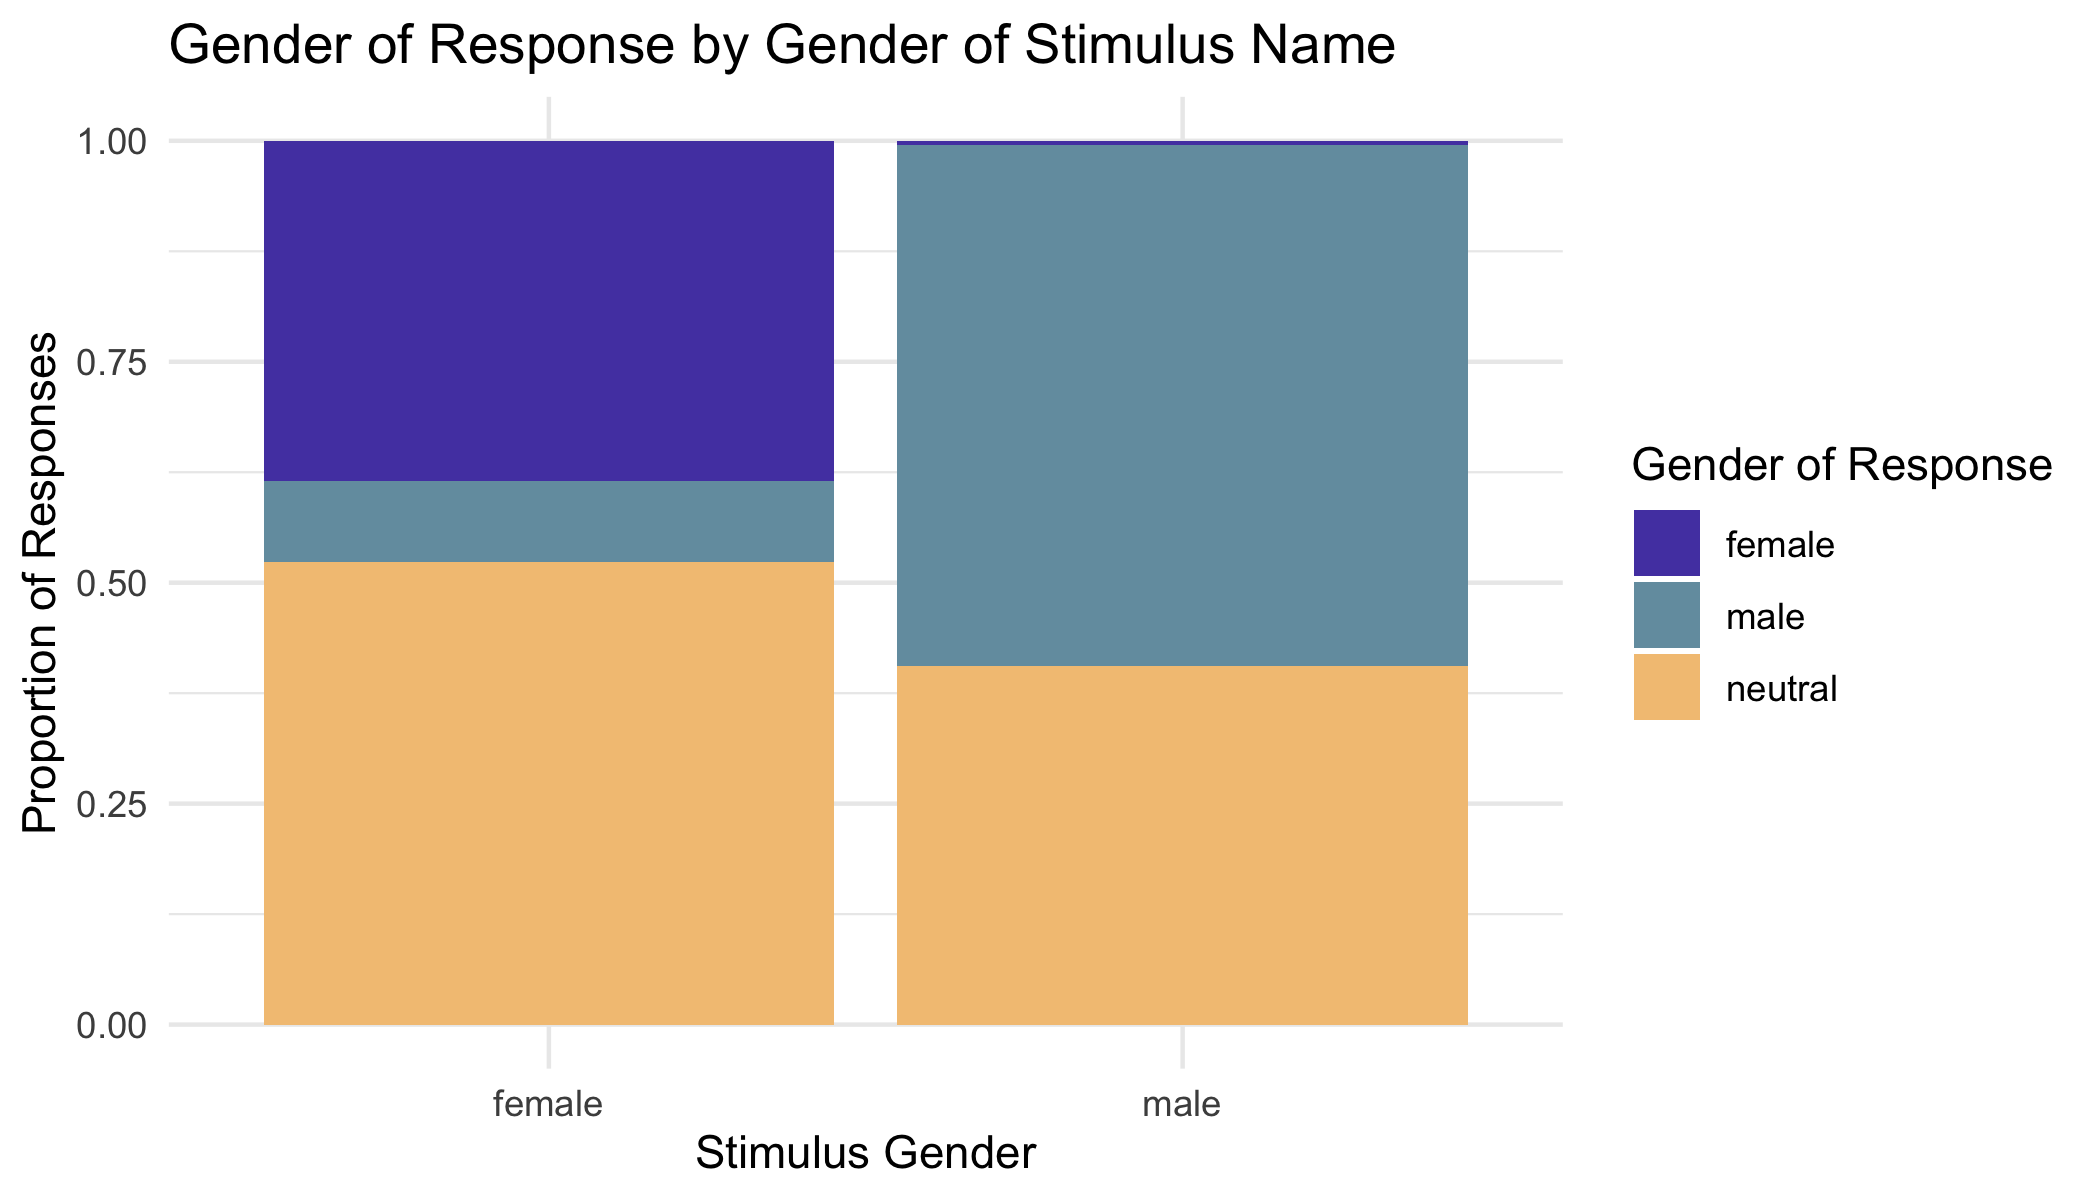
\includegraphics[scale=0.2]{prod_results_cumulative.png}
		\caption{Proportions of genders among produced responses in compound critical items}
	\end{figure}

	\begin{figure}[h!]
	\centering
	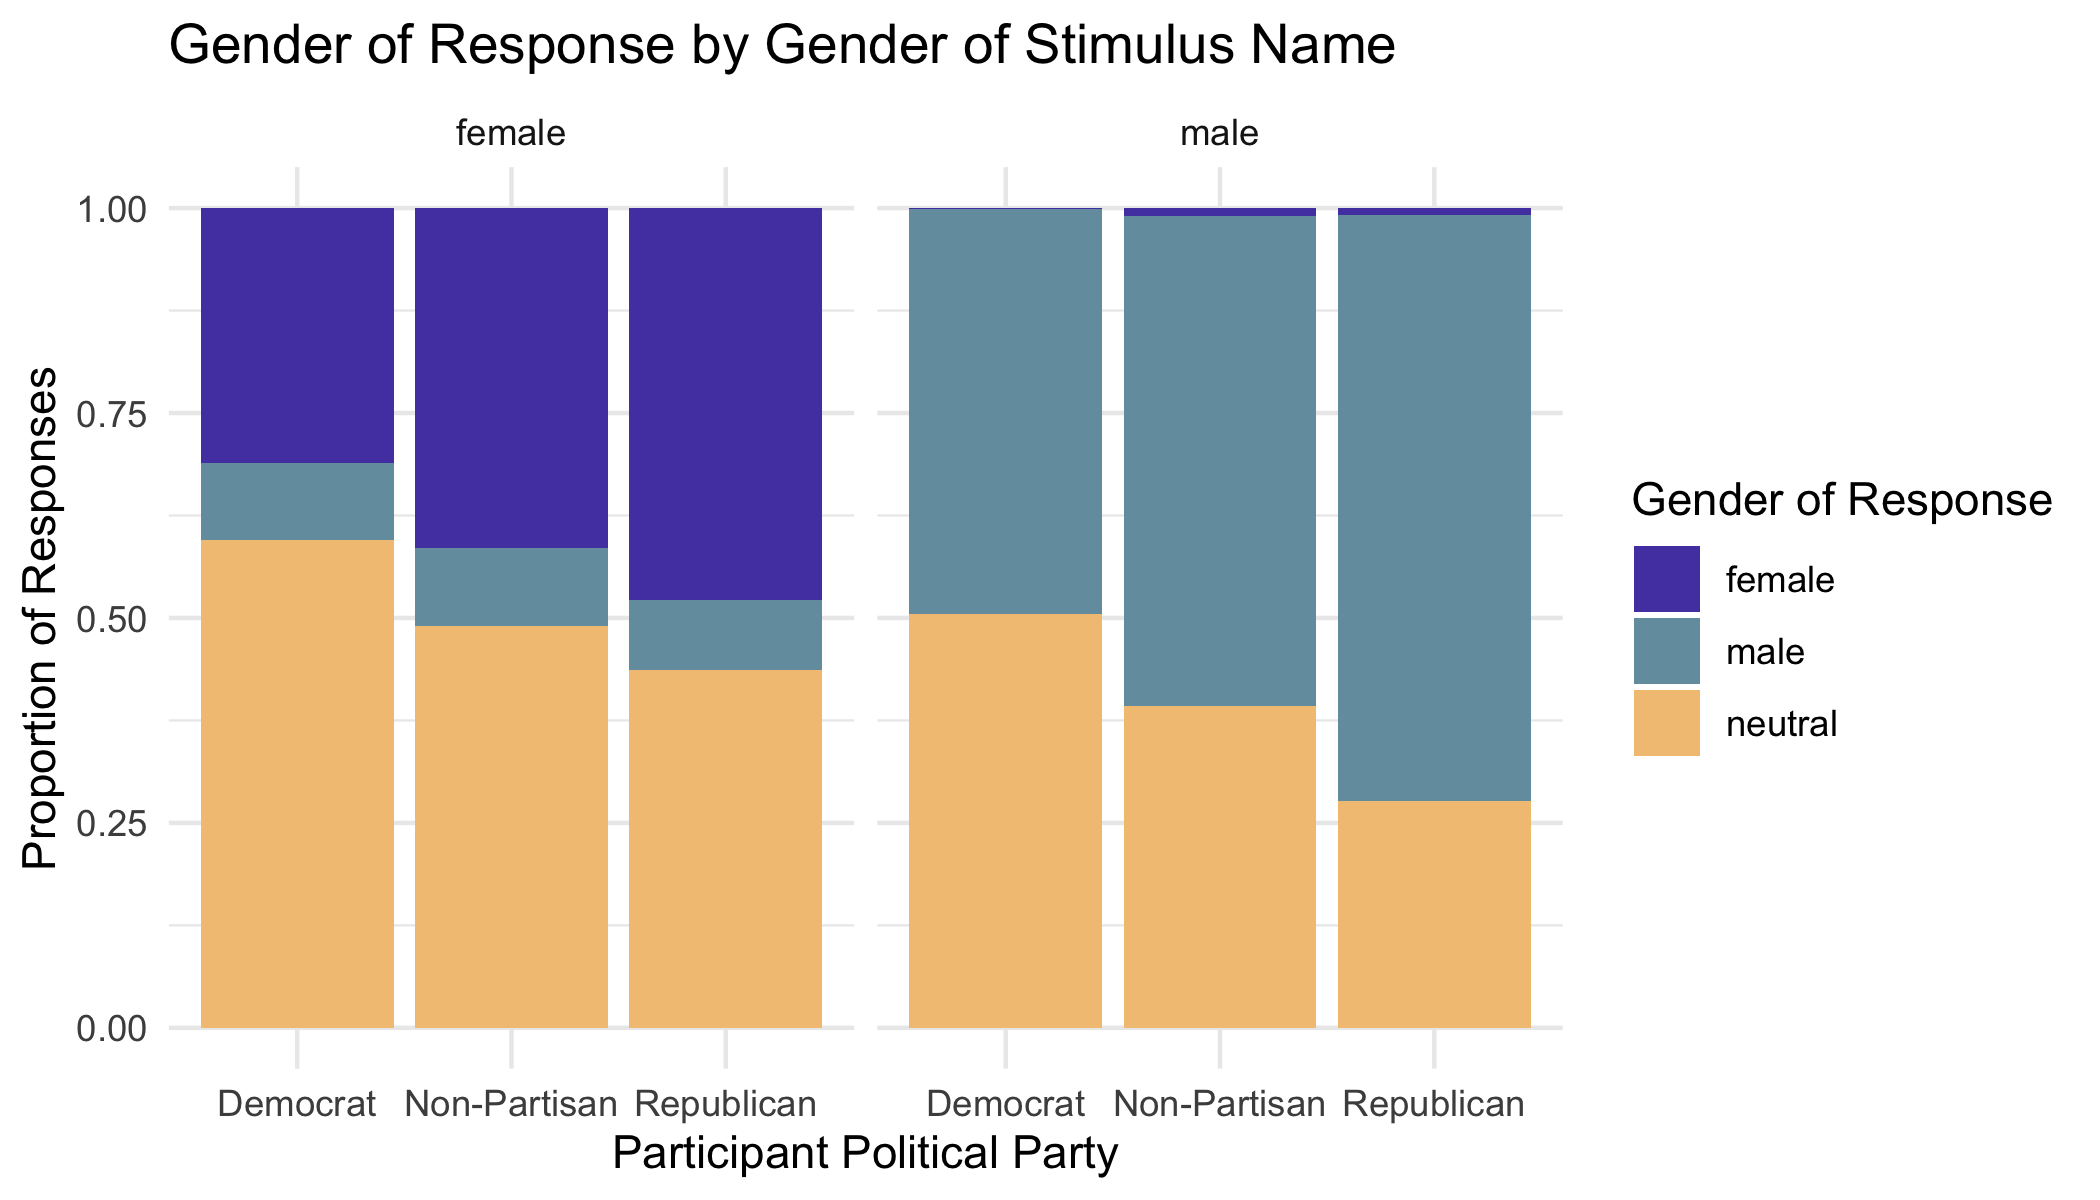
\includegraphics[scale=0.2]{prod_comp_party.png}
	\caption{Proportions of genders among produced responses in compound critical items}
	\end{figure}

	\begin{figure}[h!]
	\centering
	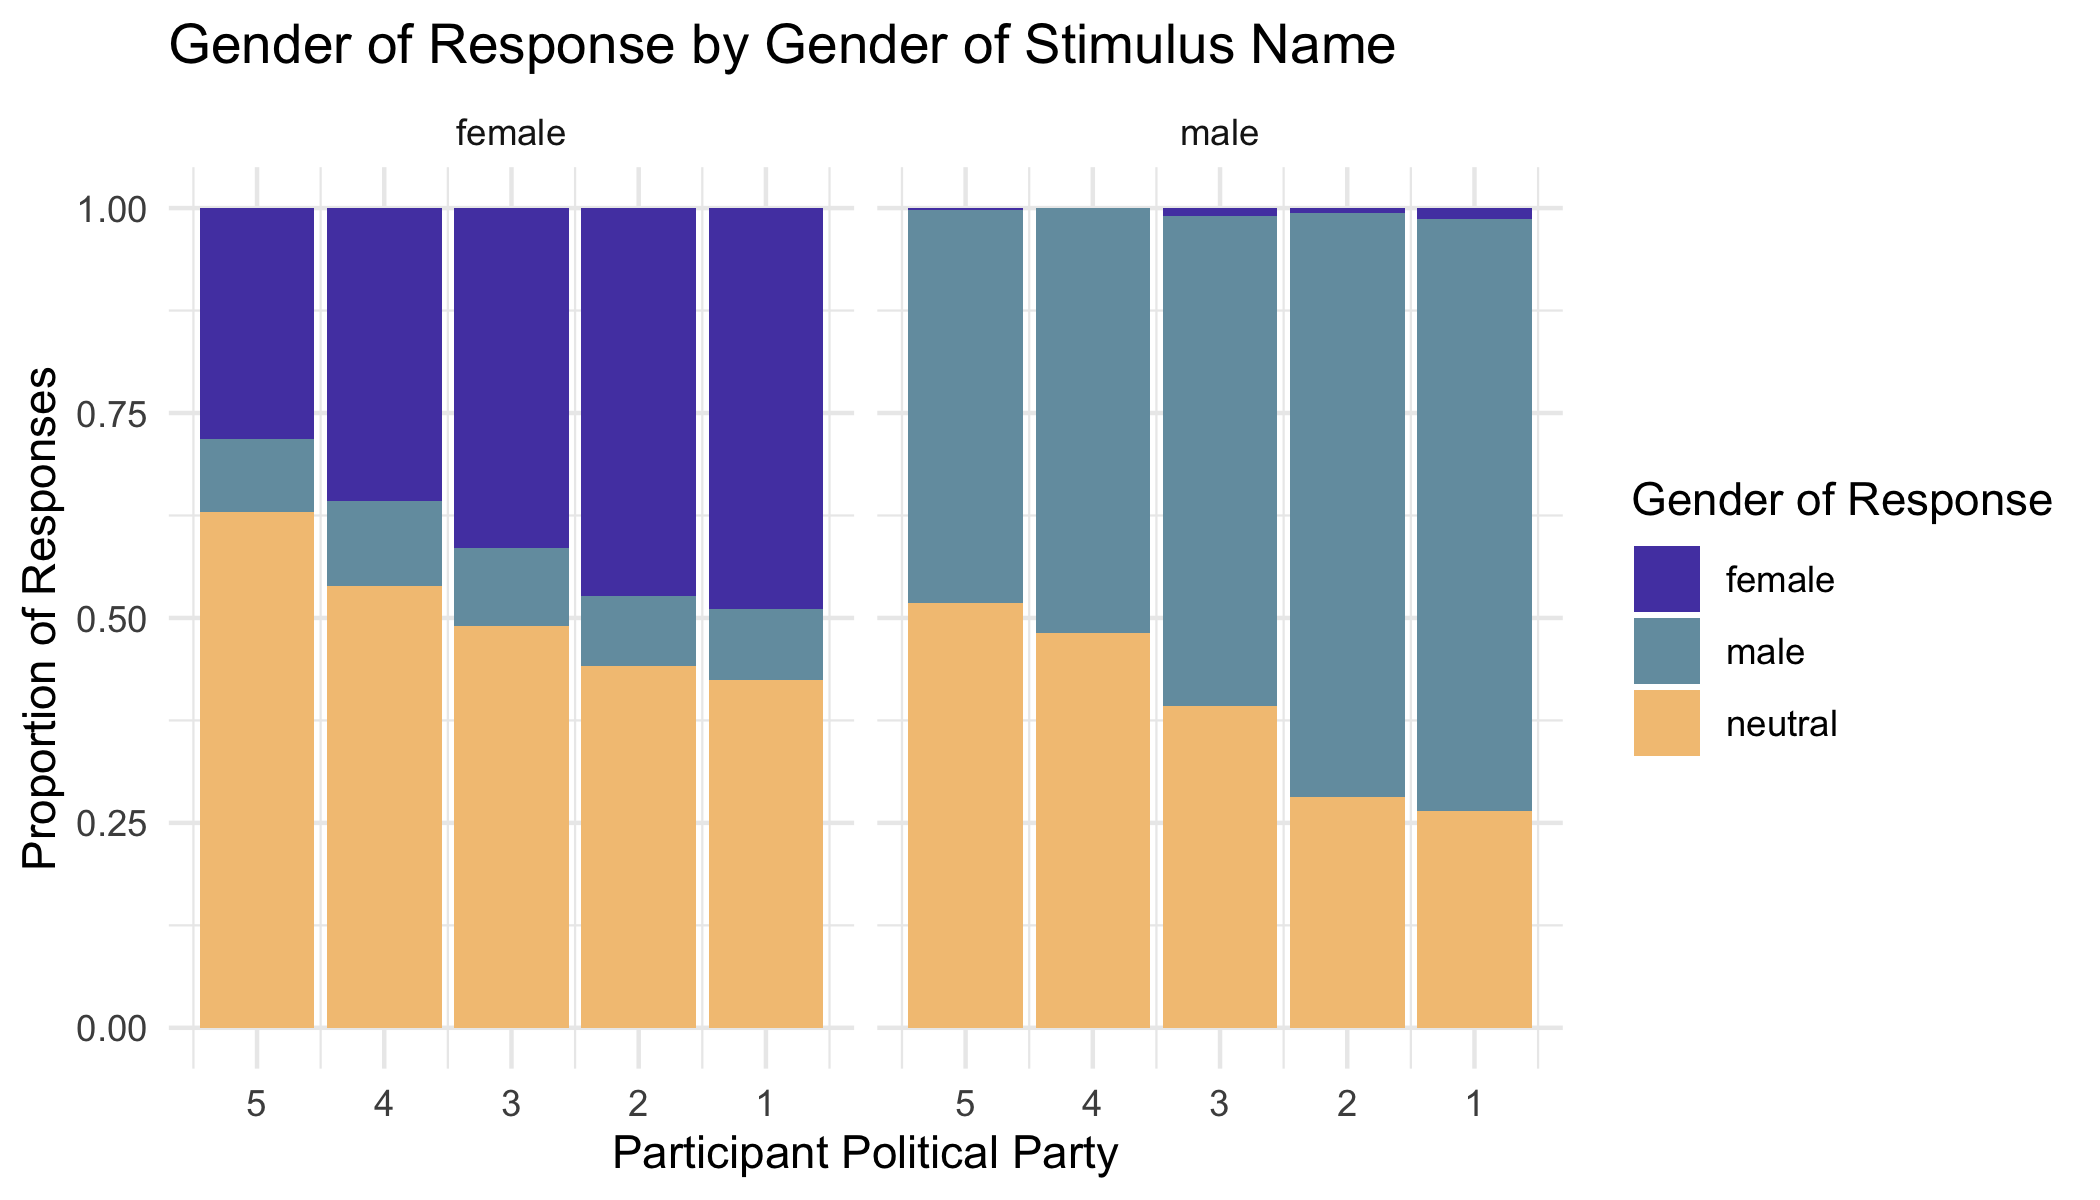
\includegraphics[scale=0.2]{prod_comp_ideo.png}
	\caption{Proportions of genders among produced responses in compound critical items}
	\end{figure}
	
	\newpage
	\section{Experiment 2}
	
	\subsection{Methods}
	
	\subsubsection{Participants}
	
	\subsubsection{Materials}
	
	\begin{table}[h!]
		\centering
		\begin{tabular}{l|l}
			\textbf{Condition} & \textbf{Example Stimulus}\\
			\hline
			Male-Congruent & \textit{David is a congressman from Virginia. He likes cycling.} \\
			Male-Neutral & \textit{David is a congressperson from Virginia. He likes cycling.} \\
			Female-Congruent & \textit{Sally is a congresswoman from Virginia. She likes cycling.}\\
			Female-Neutral & \textit{Sally is a congressperson from Virginia. She likes cycling.}
		\end{tabular}
		\caption{Example stimuli from experiment}
		\label{Table1}
	\end{table}
	
	\subsubsection{Procedure}
	
	\subsection{Results}
	
	\newpage
	\section{Experiment 2.5}
	
	\subsection{Methods}
	
	\subsubsection{Participants}
	
	\subsubsection{Materials}
	
	\subsubsection{Procedure}
	
	\subsection{Results}
	
	\newpage
	\section{Experiment 3}
	
	\subsection{Methods}
	
	\subsubsection{Participants}
	
	\subsubsection{Materials}
	
	\subsubsection{Procedure}
	
	\subsection{Results}
	
	\newpage
	\section{Analysis}
	
	\newpage
	\section{Discussion}
	
	\subsection{Limitations}
	
	\subsubsection{Demographic Limitations}
	\textbf{Political Skew} \\
	\linebreak
	\textbf{Gender Skew (TikTok)}
	On 24th July, 2021, Tik Tok user @sarahndom posted a video explaining how she made extra money participating in experiments and surveys via Prolific.co, the same recruitment platform we used. \parencite{sarahndom}. As a result, Prolific saw a large spike in participant sign-ups, most of whom were young women \parencite{prolific}. The effect of this event was that our sample in the production experiment (Experiment 1) was significantly skewed towards this demographic, only 27 of 200 participants identified as male.   \par 
	This is concerning, considering the explicitly gendered nature of this work, and the consistent finding that women have more open-minded approaches to gender and its related phenomena [CITATIONS NEEDED]. 
	
	\begin{figure}[h!]
		\centering
		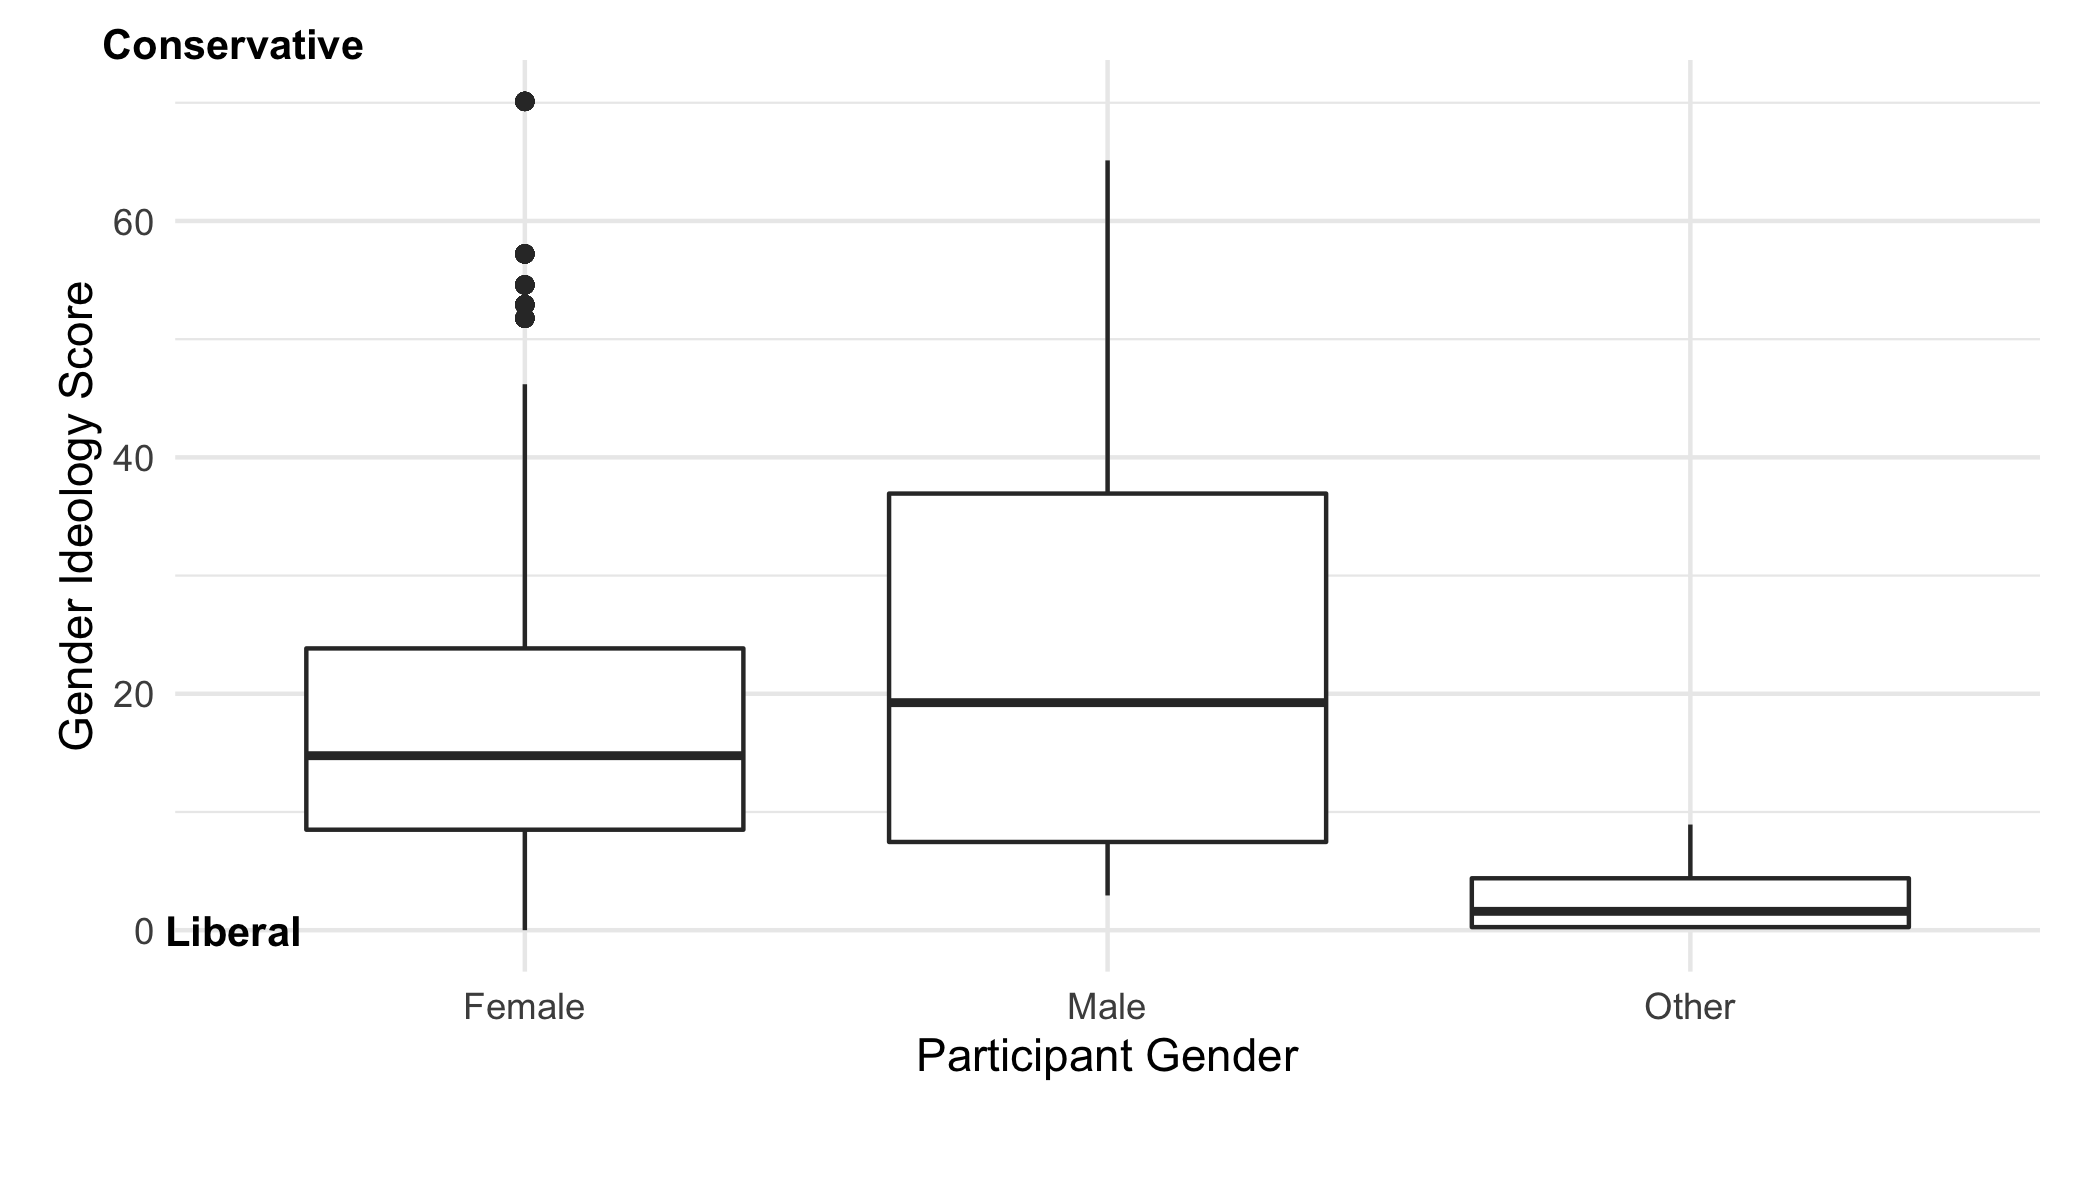
\includegraphics[scale=0.175]{prod_ideo_pure.png}
	\end{figure}
	
	\begin{figure}[h!]
		\centering
		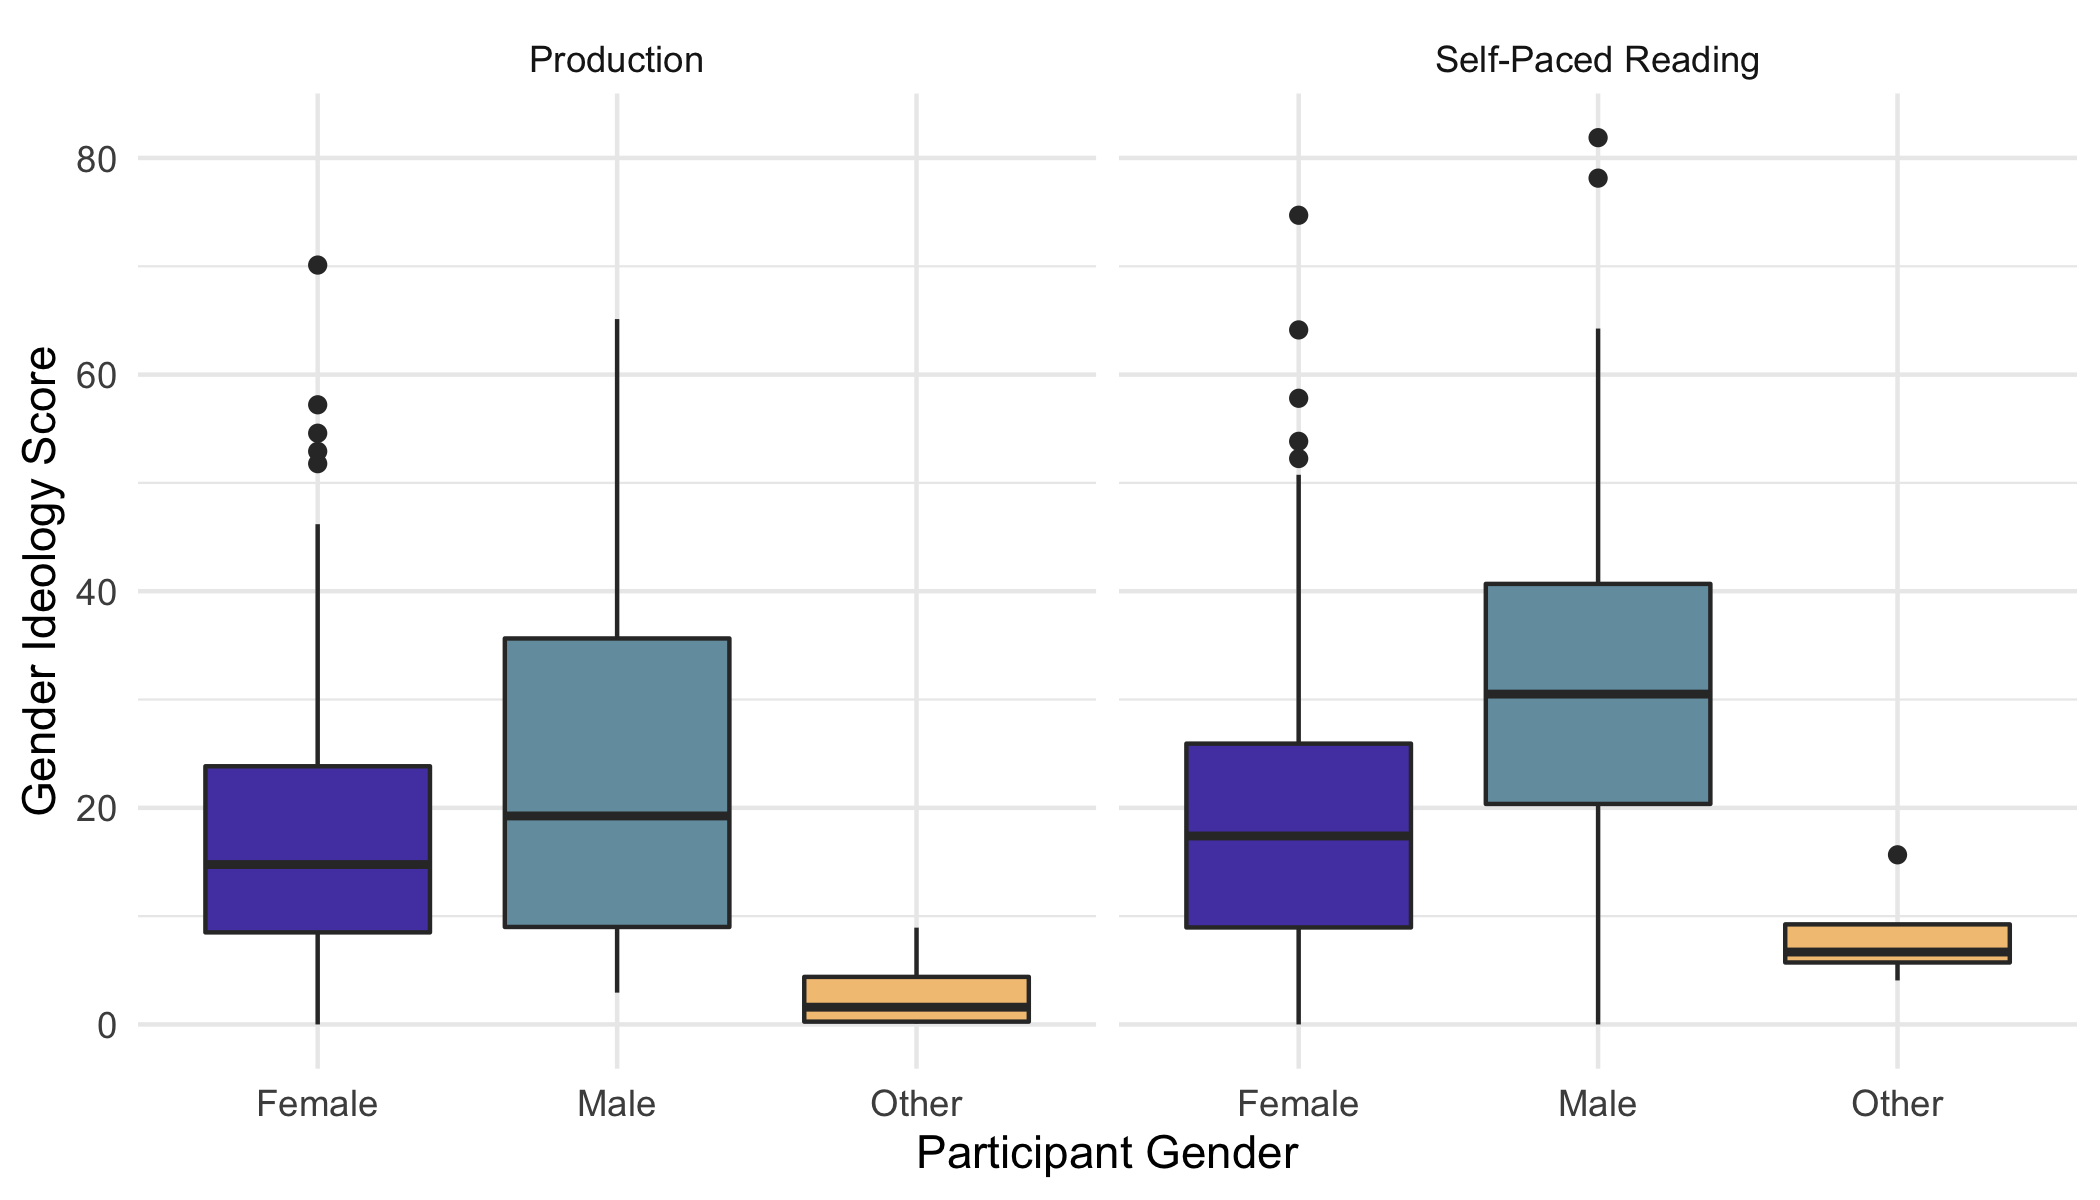
\includegraphics[scale=0.175]{merge_ideo_pure.png}
	\end{figure}
	
	\subsubsection{Stimuli Limitations}
	\textbf{Semantic Inconsistencies} \\
	\linebreak
	\textbf{Ordering of Experiment Parts}\\
	\linebreak
	\textbf{Low-Frequency Items}\\
	\linebreak
	\textbf{White Names}
	
	\subsubsection{Analysis Limitations}
	\textbf{Age-Ideology Confound}\\
	\linebreak
	\textbf{Colinearity in Normed Values}
	
	\subsection{Future Directions}
	
	\begin{itemize}
		\item Crossing raced names with gendered name
	\end{itemize}
	
	\newpage
	\section{Conclusion}
	
	\newpage
	
	\section*{Appendices}
	\addcontentsline{toc}{section}{\numberline{}Appendices}
	
	\subsection*{Appendix A: Critical Items for Norming Study}
	\addcontentsline{toc}{subsection}{\numberline{}Appendix A: Critical Items for Norming Study}
	
	\begin{table}[h!]
		\centering
		\begin{tabular}{|l|l|l|l|}
			\hline
			\textbf{Lexical Item} & \textbf{Male} & \textbf{Neutral} & \textbf{Female} \\
			\hline
			Actor & \multicolumn{2}{c|}{actor} & actress \\
			\hline
			Anchor & anchorman & anchor & anchorwoman \\
			\hline
			Assembly- & assemblyman & assemblyperson & assemblywoman \\
			\hline
			Bar- & barman & bartender & barmaid \\
			\hline
			Business- & businessman & businessperson & businesswoman \\
			\hline
			Camera- & cameraman & camera operator & camerawoman \\
			\hline
			Chair- & chairman & chair & chairwoman \\
			\hline
			Congress- & congressman & congressperson & congresswoman \\
			\hline 
			Crafts- & craftsman & craftsperson & craftswoman \\
			\hline 
			Crew- & crewman & crewmember & crewwoman \\
			\hline
			Door- & doorman & door attendant & doorwoman \\
			\hline
			Emperor & \multicolumn{2}{c|}{emperor} & empress \\
			\hline 
			Fire- & fireman & firefighter & firewoman \\
			\hline
			Fisher- & fisherman & fisher & fisherwoman \\
			\hline
			Flight & steward & flight attendant & stewardess \\
			\hline
			Fore- & foreman & foreperson & forewoman \\
			\hline
			Garbage- & garbageman & garbage collector & garbagewoman \\
			\hline
			Gentle- & gentleman & gentleperson & gentlewoman \\
			\hline
			God- & \multicolumn{2}{c|}{god} & goddess \\
			\hline
			Head- & headmaster & headteacher & headmistress \\
			\hline
			Heir & \multicolumn{2}{c|}{heir} & heiress \\
			\hline 
			Hero & \multicolumn{2}{c|}{hero} & heroine \\
			\hline
			Horse- & horseman & horseperson & horsewoman \\
			\hline
			Host & \multicolumn{2}{c|}{host} & hostess \\
			\hline
			Hunter & \multicolumn{2}{c|}{hunter} & huntress \\
			\hline
			Lay- & layman & layperson & laywoman \\
			\hline
			Mail- & mailman & mail carrier & mailwoman \\
			\hline 
			Maintenance & handyman & maintenance person & handywoman \\
			\hline 
			Weather- & weatherman & meteorologist & weatherwoman \\
			\hline 
			News- & \multicolumn{2}{c|}{newsboy} & newsgirl \\
			\hline
			Paper- & paperboy & paper carrier & papergirl \\
			\hline 
			Police- & policeman & police officer & policewoman \\
			\hline
			Land- & landlord & proprietor & landlady \\
			\hline
			Wait- & waiter & restaurant server & waitress \\
			\hline 
			Sales- & salesman & salesperson & saleswoman \\
			\hline 
			Sorce- & \multicolumn{2}{c|}{sorcerer} & sorceress \\
			\hline
			Stunt- & stuntman & stunt double & stuntwoman \\
			\hline 
			Usher- & \multicolumn{2}{c|}{usher} & usherette \\
			\hline 
			Villain- & \multicolumn{2}{c|}{villain} & villainess \\
			\hline
					
		\end{tabular}
	\end{table}
	
	\newpage
	
		\subsection*{Appendix B: Critical Items for Self-Paced Reading, Maze, and Production Tasks}
		
	\addcontentsline{toc}{subsection}{\numberline{}Appendix AB Critical Items for Self-Paced Reading, Maze, and Production Tasks}		
	
	\begin{table}[h!]
		\centering
		\begin{tabular}{|l|l|l|l|}
			\hline
			\textbf{Lexical Item} & \textbf{Male} & \textbf{Neutral} & \textbf{Female} \\
			\hline
			Actor & \multicolumn{2}{c|}{actor} & actress \\
			\hline
			Anchor & anchorman & anchor & anchorwoman \\
			\hline
			Business- & businessman & businessperson & businesswoman \\
			\hline
			Camera- & cameraman & camera operator & camerawoman \\
			\hline
			Congress- & congressman & congressperson & congresswoman \\
			\hline 
			Crafts- & craftsman & craftsperson & craftswoman \\
			\hline 
			Crew- & crewman & crewmember & crewwoman \\
			\hline
			Fire- & fireman & firefighter & firewoman \\
			\hline
			Flight & steward & flight attendant & stewardess \\
			\hline
			Fore- & foreman & foreperson & forewoman \\
			\hline
			Heir & \multicolumn{2}{c|}{heir} & heiress \\
			\hline 
			Hero & \multicolumn{2}{c|}{hero} & heroine \\
			\hline
			Host & \multicolumn{2}{c|}{host} & hostess \\
			\hline
			Hunter & \multicolumn{2}{c|}{hunter} & huntress \\
			\hline
			Lay- & layman & layperson & laywoman \\
			\hline
			Weather- & weatherman & meteorologist & weatherwoman \\
			\hline 
			Police- & policeman & police officer & policewoman \\
			\hline
			Sales- & salesman & salesperson & saleswoman \\
			\hline
			Stunt- & stuntman & stunt double & stuntwoman \\
			\hline 
			Villain- & \multicolumn{2}{c|}{villain} & villainess \\
			\hline
			
		\end{tabular}
	\end{table}
	
	
	\newpage
	\nocite{kelly2018}
	\printbibliography
	
\end{document}